% Chapter 1

\chapter{Introducción general}
\label{Chapter1}
\label{IntroGeneral}

En el presente capítulo se contextualiza la detección de anomalías en servicios de televisión por protocolo de internet (TV-over-IP) \citep{itu_iptv_overview}. Se revisa el estado del arte de forma breve y se enuncian los objetivos del trabajo.

\section{Introducción general al tema}

Los servicios de video bajo demanda y de transmisión lineal sobre redes IP consolidaron en la última década un modelo en que la calidad percibida por el usuario depende tanto de la disponibilidad de los componentes de \textit{backend} como del desempeño de la cadena completa: balanceadores, microservicios, bases de datos, colas de mensajes y sistemas de caché, entre otros. La operación de estos sistemas se apoya de manera casi universal en la recolección periódica de métricas técnicas (latencias, tasas de error, uso de CPU o memoria, etc.) que describen el estado del servicio en el tiempo.

En un servicio de TV-over-IP, el contenido audiovisual se origina en sistemas de producción o almacenamiento \citep{itu_iptv_overview}, se distribuye a través de redes de entrega y se expone al usuario final mediante aplicaciones o decodificadores físicos. Cualquier eslabón de esa cadena puede degradar la experiencia de visualización aunque el resto del sistema siga respondiendo.

Un origen saturado, un cuello de botella en la entrega o una API lenta se manifiestan para el espectador como interrupciones, demoras en el arranque de la reproducción o pérdida de calidad percibida. 

Desde el punto de vista operativo, las degradaciones relevantes suelen adoptar formas reconocibles: incrementos sostenidos de latencia, picos en la tasa de errores, caídas abruptas de la capacidad de atención simultánea o combinaciones de esas señales que no coinciden con un único síntoma aislado.

El \textit{machine learning} aporta métodos que aprenden, a partir de datos históricos, qué aspecto tiene el comportamiento nominal sin fijar a priori todas las reglas. En particular, las redes neuronales recurrentes con unidades de memoria a largo plazo (LSTM, por sus siglas en inglés) permiten modelar dependencias temporales en series multivariadas \citep{hochreiter1997long}. Los \textit{autoencoders} basados en LSTM pueden entrenarse para reconstruir ventanas recientes de métricas. Cuando la reconstrucción falla de manera sistemática, el error sirve como señal de anomalía \citep{malhotra2015long}. Este tipo de enfoque es comprensible para un lector familiarizado con monitoreo de infraestructura aunque no especializado en aprendizaje profundo: la idea central es que el modelo aprende un patrón habitual y marca desviaciones fuertes respecto de ese patrón.

Una anomalía en este contexto operativo puede entenderse como un patrón de comportamiento en esas señales que se aparta de lo observado cuando el sistema funciona de forma nominal, ya sea por degradación, por un incidente puntual o por una combinación de factores que los umbrales convencionales no caracterizan bien.

La figura~\ref{fig:anomalia-ejemplo} ilustra esta idea sobre una métrica sintética observada a lo largo de un día: la banda verde representa el régimen nominal esperado para esa hora y la curva azul, las observaciones reales. El tramo rojo marca una ventana en la que el comportamiento se aparta del patrón habitual y representa el tipo de desvío sostenido que se busca identificar de manera automática. Detectar esas situaciones de manera temprana importa porque reduce el tiempo de detección de incidentes y acota el impacto en la experiencia de visualización y en los acuerdos de nivel de servicio.

\begin{figure}[ht]
	\centering
	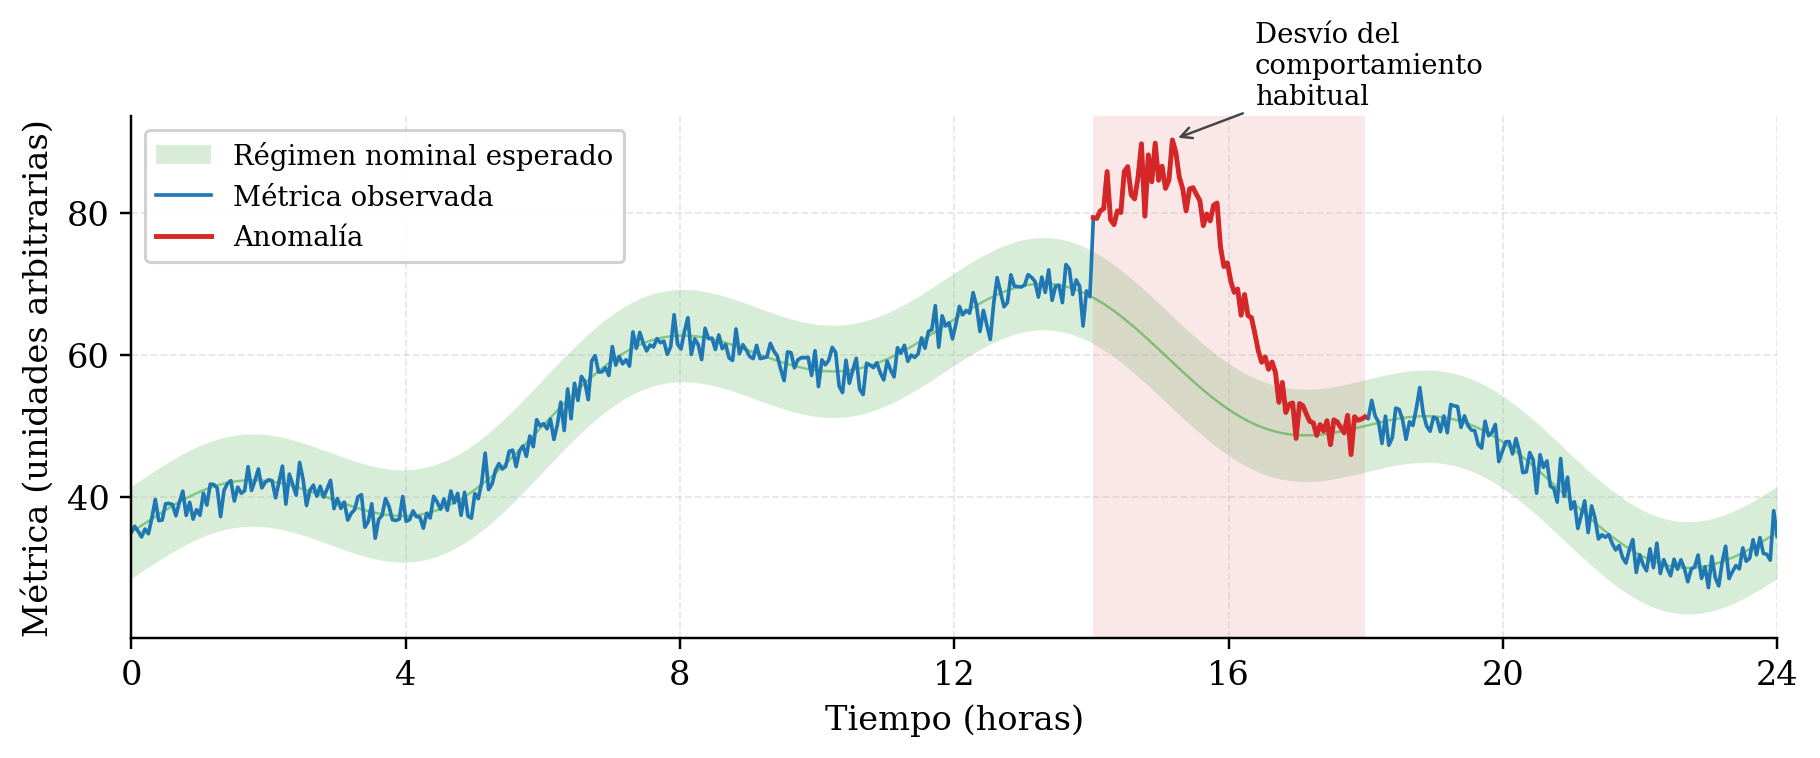
\includegraphics[width=0.85\textwidth]{./Figures/anomaly_example.png}
	\caption{Ejemplo conceptual de una métrica de servicio con un tramo de comportamiento anómalo.}
	\label{fig:anomalia-ejemplo}
\end{figure}

\section{Contexto y motivación}

La motivación del trabajo final surge de una aplicación real en el sector de plataformas de video empresarial: la organización de referencia provee servicios de TV-over-IP sobre infraestructura en la nube y requirió modernizar la forma en que se detectan fallos y degradaciones en producción. Las métricas del servicio se concentran en herramientas estándar de la industria, en particular en un sistema de acumulación de series temporales del tipo de Prometheus \citep{brazil2018prometheus, prometheus_site}, con muestreo en el orden de decenas de segundos.

Las prácticas tradicionales de alertas sobre umbrales fijos o reglas manuales siguen siendo útiles para síntomas claros, pero muestran debilidades frente a patrones multivariados, estacionalidades (por ejemplo variaciones por horario comercial o fines de semana) y dependencias que no se traducen en un único umbral intuitivo. Además, externalizar el análisis de métricas a terceros puede no ser deseable desde el punto de vista de privacidad y superficie de ataque.

En el entorno de la organización de referencia se acumularon reglas de alerta sobre muchas series en paralelo. Con el tiempo, una fracción creciente de notificaciones correspondió a situaciones que no requerían intervención inmediata o que repetían patrones estacionales ya conocidos. 

Esa carga incrementó el esfuerzo del equipo de operaciones en la priorización de incidentes y elevó el riesgo de desatender eventos realmente críticos. Los falsos positivos repetidos también afectaron la confianza en el canal de alertas y dificultaron sostener acuerdos de nivel de servicio cuando las degradaciones no se detectaban con la anticipación deseada. 

Por estas razones se buscó una detección más contextual, capaz de considerar varias señales a la vez, y se priorizó mantener la telemetría y el entrenamiento del modelo dentro del perímetro controlado por la empresa, sin depender de servicios analíticos externos para el núcleo de la detección.

Por ello se planteó un sistema integrado al monitoreo existente, orientado a procesar ventanas multivariadas y a emitir alertas contextualizadas cuando el patrón observado se aparta del régimen nominal aprendido. La integración con herramientas de observabilidad ya adoptadas permitió reutilizar la recolección y los tableros existentes. El esfuerzo de este trabajo se concentró en el núcleo analítico y en el encadenamiento hacia sistemas de respuesta a incidentes.

\section{Estado del arte}

La detección de anomalías abarca desde métodos estadísticos y basados en distancia hasta técnicas de aprendizaje profundo adaptadas a datos secuenciales. Existe una vasta literatura de marcos de referencia y taxonomías \citep{chandola2009anomaly}.

En operaciones de software, los datos son en la práctica series multivariadas en las que distintas métricas capturan facetas acopladas del sistema, lo que motiva modelos que traten la ventana temporal completa en lugar de decidir variable por variable de forma independiente, para capturar no linealidades y dependencias largas. En monitorización de aplicaciones e ingeniería de confiabilidad de sitios, la práctica habitual combina métricas de utilización, saturación y errores con umbrales declarativos. Ese enfoque resulta adecuado para síntomas univariados claros, pero pierde expresividad cuando un incidente modula en forma acoplada varias series antes de que cualquiera de ellas supere un límite fijo \citep{brazil2018prometheus}.

Los métodos clásicos (controles por umbrales, suavizados exponenciales o \textit{isolation forest} \citep{liu2008isolation} sobre vectores de características) conservan ventajas de simplicidad e interpretabilidad, pero pueden exigir mucho ajuste manual cuando el número de series crece o cuando la normalidad cambia lentamente en el tiempo. Los autoencoders y las arquitecturas recurrentes ofrecen una capa adicional de expresividad para capturar no linealidades y dependencias largas.

Entre los enfoques de aprendizaje profundo para series temporales, Malhotra et al. \citep{malhotra2015long} entrenaron redes codificadoras-decodificadoras LSTM exclusivamente con ventanas consideradas normales y utilizaron el error de reconstrucción como indicador de anomalía. Esa línea resultó aplicable al monitoreo operativo multivariado, aunque con variables y régimen de muestreo propios del dominio de \textit{streaming} empresarial. Trabajos posteriores exploraron arquitecturas con atención, convoluciones temporales o modelos generativos. Para telemetría con pocas decenas de variables y muestreo periódico fijo, un autoencoder LSTM compacto sigue siendo una base interpretable y eficiente en CPU.

Paralelamente, los ecosistemas de observabilidad comercial integran funciones de detección asistida o modelos propietarios sobre telemetría ya ingestada. Esas soluciones priorizan la integración con la plataforma, pero suelen ofrecer poco control sobre el entrenamiento, el umbral y la auditoría del modelo. 

La propuesta de este trabajo se acopla al \textit{stack} Prometheus--Grafana--Opsgenie \citep{salituro2020grafana, grafana_site, opsgenie_site} ya adoptado en la organización. Mantiene la configuración, el entrenamiento y la inferencia bajo control del operador. Así se busca un equilibrio entre sensibilidad y falsos positivos calibrable con el equipo de operaciones.

La tabla~\ref{tab:comparativa-enfoques} resume familias de enfoques y su relación típica con datos y métricas de evaluación. La tabla~\ref{tab:trabajos-referencia} sitúa de manera orientativa trabajos de referencia y la línea elegida en este trabajo. Ninguna de las dos pretende ser exhaustiva, sino ubicar la propuesta en el panorama habitual de ingeniería de confiabilidad y aprendizaje automático.

\begin{table}[H]
\centering
\caption{Comparación sintética de enfoques para detección de anomalías en métricas operativas (orientación conceptual).}
\label{tab:comparativa-enfoques}
\begin{tabular}{@{}p{0.21\textwidth}p{0.23\textwidth}p{0.21\textwidth}p{0.27\textwidth}@{}}
\toprule
\textbf{Enfoque} & \textbf{Tipo de modelo o regla} & \textbf{Datos típicos} & \textbf{Métricas de desempeño habituales} \\
\midrule
Umbrales fijos y reglas & Reglas declarativas, comparaciones con constantes & Series univariadas o pocas variables, supuestos estables & Tiempo de detección, acuerdo con incidentes conocidos, carga de falsas alertas. \\
Modelos clásicos de anomalía & Por ejemplo aislamiento, kNN, métodos estadísticos multivariados & Vectores de características por instante o ventana corta & Precisión, exhaustividad (\textit{recall}), F1 si existe etiquetado parcial. \\
Modelos secuenciales profundos & Autoencoder LSTM, otras RNN, a veces combinadas con atención & Ventanas multivariadas de series temporales & Error de reconstrucción, AUC--PR, F1 sobre eventos etiquetados. \\
Productos comerciales de observabilidad & Algoritmos propietarios, a veces combinados con reglas & Telemetría agregada en plataforma & Definidas por el proveedor con un foco en integración. \\
\bottomrule
\end{tabular}
\end{table}

\begin{table}[H]
\centering
\small
\caption{Trabajos de referencia y línea adoptada en esta memoria (orientación conceptual).}
\label{tab:trabajos-referencia}
\begin{tabular}{@{}p{0.22\textwidth}p{0.24\textwidth}p{0.22\textwidth}p{0.26\textwidth}@{}}
\toprule
\textbf{Referencia} & \textbf{Modelo o método} & \textbf{Tipo de datos} & \textbf{Señal o métrica de detección} \\
\midrule
Malhotra et al. \citep{malhotra2015long} & Codificador-decodificador LSTM & Series multivariadas de sensores & Error de reconstrucción \\
Liu et al. \citep{liu2008isolation} & Isolation forest & Vectores de características & Puntaje de anomalía \\
Propuesta de esta memoria & Autoencoder LSTM & Telemetría operativa de TV-over-IP & Error de reconstrucción y umbral calibrado \\
\bottomrule
\end{tabular}
\end{table}

\section{Objetivos del trabajo}

El objetivo general del trabajo consistió en diseñar e implementar un sistema inteligente capaz de detectar anomalías en tiempo de operación compatible con el monitoreo existente en un servicio de TV-over-IP basado en API, mediante un autoencoder LSTM entrenado sobre ventanas de métricas obtenidas desde Prometheus, con integración de alertas y enlaces de contexto con Opsgenie y Grafana, con miras a mejorar la capacidad de reacción frente a incidentes sin depender exclusivamente de umbrales estáticos ni de servicios de terceros para el núcleo analítico.

La evaluación del sistema se concibió en función de indicadores operativos verificables: tasa de falsos positivos sobre tramos considerados nominales, capacidad de señalar degradaciones acordadas con el equipo de operaciones y tiempo entre el inicio de un patrón anómalo y la emisión de la alerta. Esos criterios orientan los ensayos del capítulo correspondiente y permiten contrastar el enfoque aprendido frente a líneas base por umbrales fijos.

Los objetivos específicos, formulados de manera verificable, fueron los siguientes:

\begin{enumerate}
\item Identificar y preparar las métricas críticas del servicio disponibles vía API de Prometheus, incluyendo normalización, variables de contexto temporal (por ejemplo codificación cíclica de la hora) y construcción de ventanas deslizantes acordes al período de muestreo del entorno.
\item Entrenar y ajustar un modelo autoencoder LSTM capaz de reconstruir el comportamiento nominal del sistema y traducir el error de reconstrucción en una señal de anomalía gobernada por un umbral calibrado con el equipo de operaciones.
\item Integrar el flujo de inferencia con mecanismos de alerta y la generación de enlaces a paneles en Grafana que permitan inspeccionar el intervalo temporal asociado a cada anomalía detectada.
\item Evaluar el sistema sobre datos históricos representativos del régimen normal de operación, reportando al menos la tasa de falsos positivos y la capacidad de detección en escenarios acordados con las partes interesadas, de forma que los resultados en esta memoria permitan contrastar el desempeño frente a líneas base definidas en el capítulo de ensayos.
\end{enumerate}
